\section{Analysis}
\label{sec:analysis}





\begin{table*}[t]
% \small
    \centering
\resizebox{1\textwidth}{!}{%
\begin{tabular}{llllllll}
\toprule
Subject & Object & Pattern \#1 & Pattern \#2 & Pattern \#3 & Pred \#1 & Pred \#2 & Pred \#3 \\
\midrule

% Adam Kendon & London & [X] was born in [Y]. & [X] is originally from [Y]. & The country of origin of [X] is [Y]. & \hltrue{London} & \hltrue{London} & \hlfalseo{Ireland} \\
Adriaan Pauw & Amsterdam & [X] was born in [Y]. & [X] is native to [Y]. & [X] is a [Y]-born person. & \hltrue{Amsterdam} & \hlfalseo{Madagascar} & \hlfalset{Luxembourg} \\
Nissan Livina Geniss & Nissan & [X] is produced by [Y]. & [X] is created by [Y]. & [X], created by [Y]. & \hltrue{Nissan} & \hlfalseo{Renault} & \hlfalseo{Renault} \\
Arab League & Asia & [X] belongs to the continent of [Y]. & [X] is located in [Y]. &  [X] is a part of the continent of [Y]. & \hltrue{Asia} & \hlfalseo{Europe} & \hlfalset{Africa} \\ 
% Albania & Serbia & [X] shares border with [Y]. & [Y] borders with [X]. & [Y] shares the border with [X] & \hlfalseo{Greece} & \hlfalset{Turkey} & \hlfalsetr{Kosovo} \\
iCloud & Apple & [X] is developed by [Y]. & [X], created by [Y]. & [X] was created by [Y] & \hlfalseo{Microsoft} & \hlfalset{Google} & \hlfalsetr{Sony} \\
\midrule

Yahoo! Messenger & Yahoo & [X], a product created by [Y] & [X], a product developed by [Y] & [Y], that developed [X] & \hlfalseo{Microsoft} & \hlfalseo{Microsoft} & \hlfalseo{Microsoft} \\
Wales & Cardiff & The capital of [X] is [Y] . & [X]'s capital, [Y]. & [X]'s capital city, [Y]. & \hltrue{Cardiff} & \hltrue{Cardiff} & \hltrue{Cardiff} \\

\bottomrule
\end{tabular}


}
    \caption{Predictions of BERT-large-cased. Presenting the
      subjects and objects taken from T-REx \cite{trex}, as
      well as three different patterns from our resource and
      their predictions. The predictions are colored in blue
      if the model predicted correctly (out of the candidate
      list), and in red otherwise. If there is more than a
      single erroneous prediction, it is colored by a different red.}
    \label{tab:predictions}
\end{table*}


\subsection{Qualitative Analysis}
In order to better understand the factors affecting consistent predictions, we inspect the predictions of BERT-large on different patterns, which are summarized in Table \ref{tab:predictions}.
We highlight several cases.
The predictions in the first row are inconsistent, and
correct for the first pattern, but not for the other two. 
The predictions in the second row also show a single pattern that predicted the right object, however, the two other patterns, which are lexically similar, predicted the same, wrong answer - Renault.
% However, the third pattern prediction is related in the sense that Ireland is close to London. \ye{is the Ireland-London argument convincing?}
% The last row of the upper part detail three different incorrect predictions. 
% Note that the patterns of the penultimate row predicted two factually correct answers out of three (Greece, Kosovo), but simply do not correspond to the gold object in T-REx (Albania), since this is an M-N relation. 
The last row of the upper part demonstrates three different predictions, all factually incorrect. 
% Note that even when more than a single answer is correct, we still argue that the model should make consistent predictions.
Finally, the predictions in the bottom part demonstrate
consistent predictions:
The last row  is consistent and factual, the last but one
row is consistent, but factually incorrect (surprisingly due to the fact the object is a substring of the subject).





\begin{figure}[t!]
\centering

% \subfloat{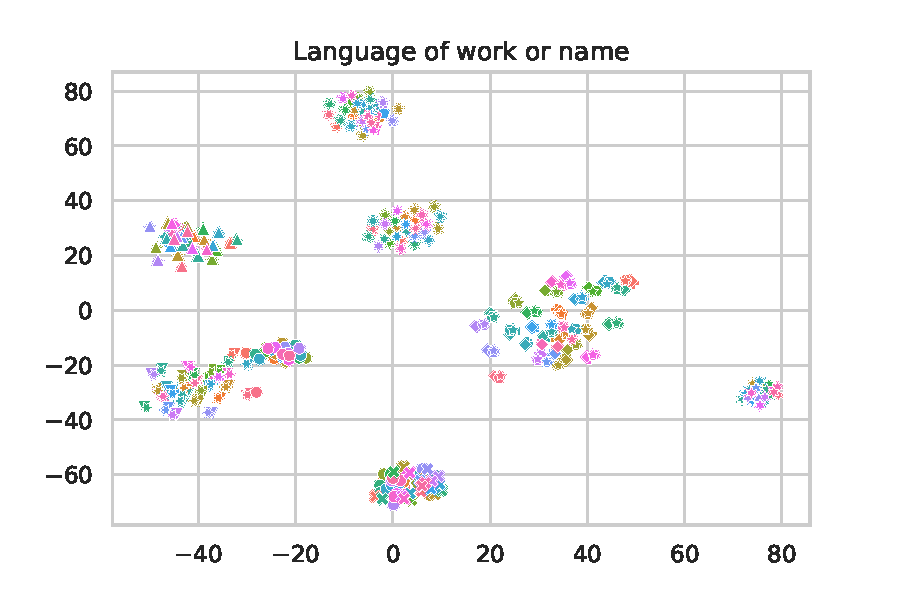
\includegraphics[width=1.\columnwidth]{figures/P407_emb.pdf}}\\
%   \hfill
\subfloat{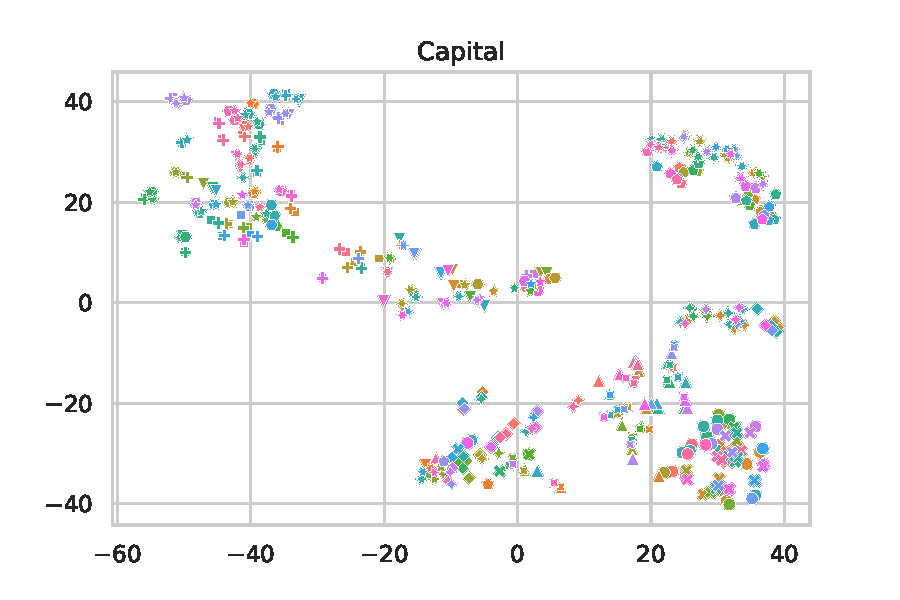
\includegraphics[width=1.\columnwidth]{figures/capital-bert-large}}
% \\


\caption{t-SNE plots for encoded patterns from the
  \textit{capital} relation. Points of the same color
  represent the same subject, points of the same shape
  represent the same pattern. We expect that a knowledge-focused representation  clusters based on identical-subjects (color) rather than identical-patterns (shape).}
\label{fig:tsne-emb}

\end{figure}

\subsection{Representation Analysis}


To provide insights on the models' representations, we inspect these after encoding the cloze-style patterns.

Motivated by previous work that found that words with the same syntactic structure cluster together \cite{chi-etal-2020-finding,ravfogel-etal-2020-unsupervised} we perform a similar experiment to test if this behavior replicates with respect to knowledge:
We encode the patterns, after filling the placeholders with subjects and masked tokens and inspect the last layer representations in the masked token position.
When plotting the results using t-SNE \cite{tsne} we mainly
observe clustering based on the patterns, which suggests
that
%the knowledge, therefore the
encoding of knowledge of the entity is not the main component of the representations.
Figure \ref{fig:tsne-emb} demonstrates
%such graph
this
for BERT-large encodings of the \textit{capital} relation.\footnote{While some patterns are clustered based on the subjects in the top-left part, most of them are clustered based on pattern.}
\enote{hs}{following sentences: i didn't understand how the
  clustering is done}
We also cluster these representations using two different number of centroids:\footnote {Using the KMeans algorithm} (1) the number of patterns in each relation and (2) the number of entities in each relation. We then measure the purity of these clusters using V-measure. We observe that the clusters are mostly grouped by the patterns, rather than the objects.
% Finally, we compute the correlation between the distance of two representations, and whether their predictions are consistent. 
Finally, we compute the spearman correlation between the consistency scores and the v-measure of the representations.
However, the correlation between these variables is low (close to zero, and not significant)\footnote{Except for BERT-large whole-word-masking, where the correlation is 39.5 ($p-val<0.05$).}, therefore not explaining the models' behavior.
This finding is interesting since it means that (1) these representations are not knowledge-focused, i.e. Their main component does not relate to knowledge, and (2) the entire representation does not explain the behavior of the model. This finding is consistent with previous work that observed similar trends for linguistic tasks \cite{amnesic_probing}.
We hypothesize that this disparity between the representation and the behavior of the model may be explained by a situation where distances between representations largely do not reflect the distance between predictions, but rather reflect other, behaviorally-irrelevant factors of each sentence.
% We believe that the explanation of these findings is that the relevant information for the word prediction, lies in a subspace of the original representation, and thus much of the encoded information is in practice not relevant for the prediction. \sr{I don't understand this explanation. I'd write something like ``We hypothesize that this disparity between representation and behavior may be explained by a situation where distances between representations largely do not reflect the distance between predictions, but rather reflect other, behaviorally-irrelevant factors of each sentence"}.


% We encode the patterns, populated with 50 random subjects along with the masked token, and inspect the final layer in the masked token index for all the paraphrases of multiple relations.
% Then, we use t-SNE \cite{tsne} and present the results in Figure \ref{fig:tsne-emb} in the appendix.
% Each point represents a specific tuple, and are colored by the subjects, and the shape stands for the pattern.
% A good representation would cluster the vectors together based on the subject, as then the predictions would more likely to be consistent. However, clusters based on patterns would suggest a worse encoding, since the subjects, which are of great importance in these paraphrases, are less taken into account in the representation.

% We display the t-SNE figures for two relations, \textit{Language  of work or name} and \textit{Capital} in Figure \ref{fig:tsne-emb}.
% It is clear that the first figure clusters mainly on the patterns, whereas the second figure clusters mainly on the subjects. These results are also consistent with the performance of these relations: @@\% and @@\%, which suggests a better representation for the latter.
% Additionally, we also perform clustering for the representations,\footnote{Using the KMeans algorithm.} once with the number of subjects and once with the number patterns, given as an oracle, hoping to fit the subjects or patterns clusters. Then, we calculate the v-measure metric for measuring the purity of each cluster.
% A higher score on the subject-based would suggest a representation that better fits the purpose of a KB.
% The v-measure results for these patterns are presented in Table \ref{tab:vmeasure-small}.
% As expected, the pattern-based clustering is better for the \textit{language of work or name} relation is higher than the subject-based, and vice versa for the \textit{capital} relation.
% The full clustering measures for all relations are reported in the Appendix.
% \ar{Can we report correlation with performance for all relations here? Or say that in general we observe this trend?}
% \begin{table}[t]
% \small
    \centering
% \resizebox{1\textwidth}{!}{%
\begin{tabular}{lrr}
\toprule
                                          Pattern &  pattern &  subject \\
\midrule
     language of work or name &            0.72 &            0.24 \\
                      capital &            0.41 &            0.62 \\
\bottomrule
\end{tabular}

% }
    \caption{V-measure clustering performance for the two relations. Reporting the results for clustering based on the pattern, and based on the subjects.}
    \label{tab:vmeasure-small}
\end{table}


